\section{基于深度学习的乳腺癌超声图像诊断系统设计与实现}

本章详细描述基于深度学习的乳腺癌超声图像自动诊断系统的整体设计方案与具体实现。首先介绍系统的总体架构和各模块的功能划分；然后阐述数据处理流程，包括数据集介绍、预处理操作、数据集划分策略以及DAGAN合成数据的生成方法；接着详细说明分类模型的设计方案，包括骨干网络选择、迁移学习配置、损失函数设计和训练策略优化；最后介绍Grad-CAM可解释性模块和测试时增强（TTA）推理方法的实现细节。


\subsection{系统总体架构}

本课题设计的乳腺癌超声图像自动诊断系统采用模块化的软件架构，主要由四个核心功能模块组成：

（1）\textbf{数据预处理模块}：负责原始乳腺超声图像的加载、清洗、尺寸归一化、标准化等预处理操作，以及训练集/验证集/测试集的分层划分和数据增强变换。

（2）\textbf{分类模型模块}：系统的核心模块，基于预训练的卷积神经网络（EfficientNet-B0或ResNet18），通过迁移学习实现良性、恶性、正常三分类功能。

（3）\textbf{DAGAN合成数据增强模块}：利用深度卷积生成对抗网络为训练集生成高质量合成样本，扩充训练数据量并缓解类别不平衡问题。

（4）\textbf{Grad-CAM可解释性模块}：对分类模型的预测结果生成热力图可视化，展示模型做出决策时所关注的关键区域，提供可解释的诊断依据。

系统的整体处理流程如图\ref{fig:system_architecture}所示。输入的乳腺超声图像经过预处理后送入分类模型进行推理，输出三分类预测结果及各类别置信度；同时，Grad-CAM模块对最后一个卷积层的特征图进行梯度加权计算，生成热力图并叠加于原图上进行可视化展示。

\begin{figure}[htb]
    \centering
    % 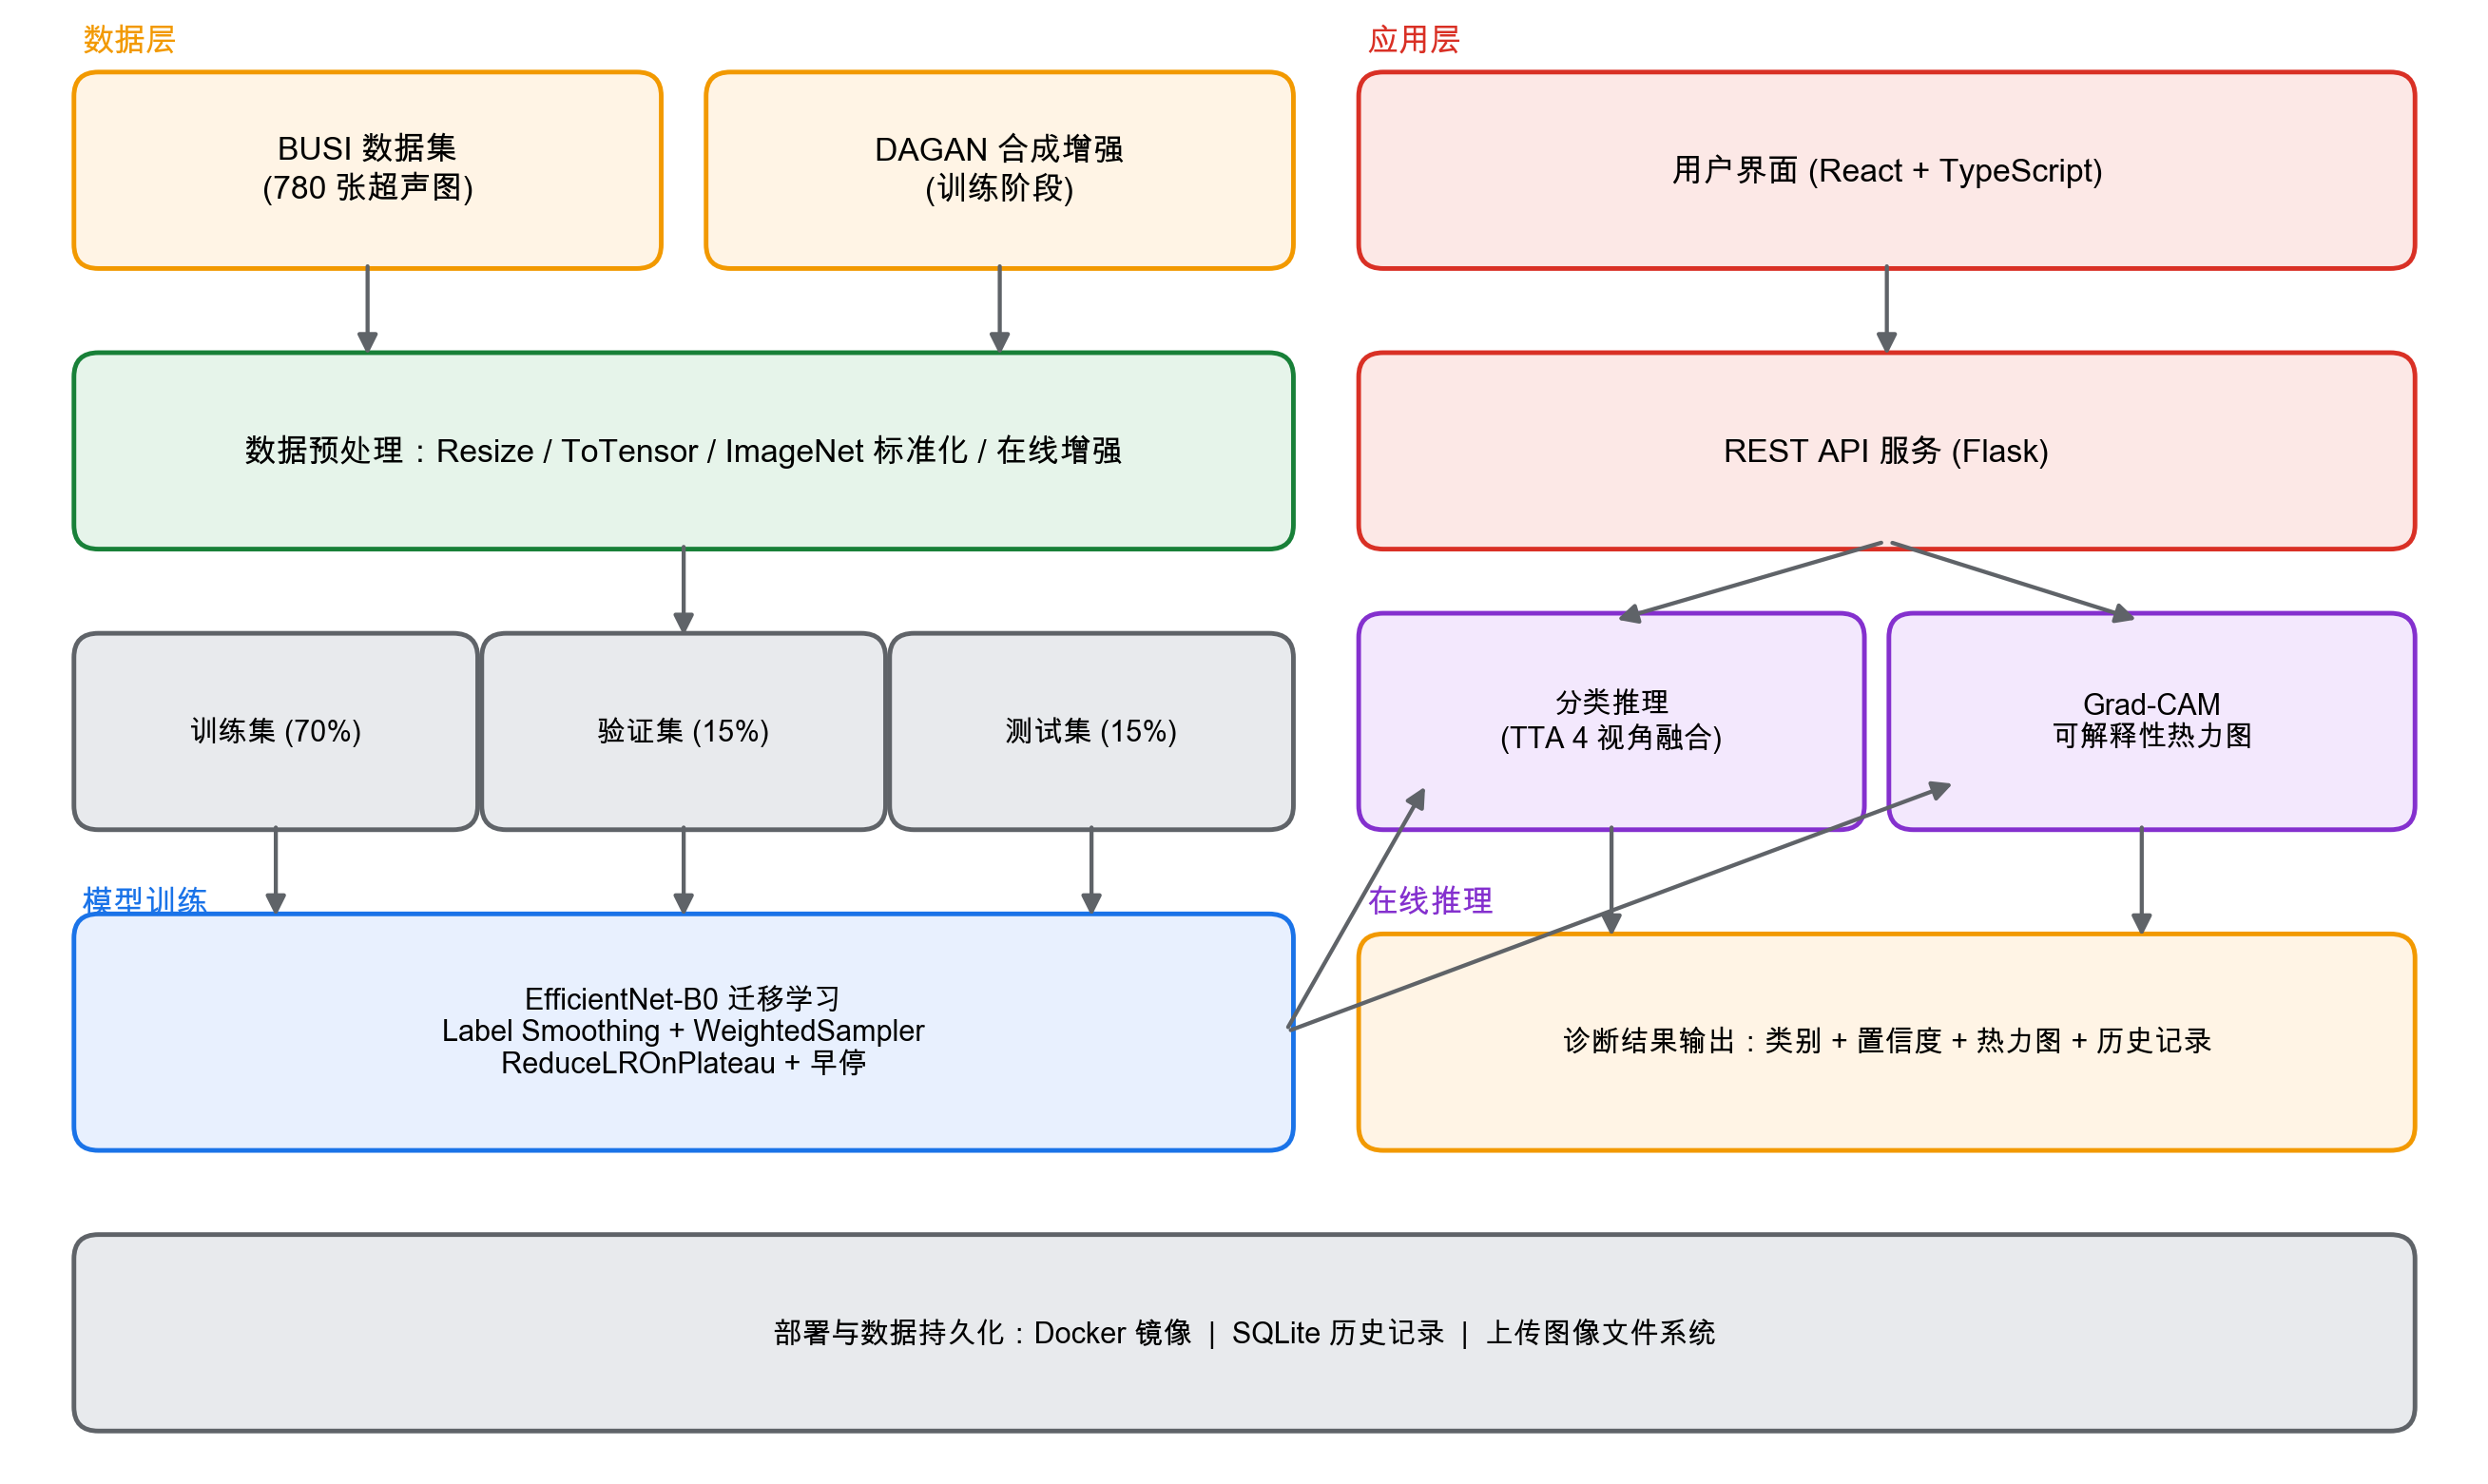
\includegraphics[width=0.85\textwidth]{images/system_architecture.png}
    \fbox{\parbox{0.8\textwidth}{\centering\vspace{2cm}系统架构图（待插入）\vspace{2cm}}}
    \caption{乳腺癌超声图像自动诊断系统总体架构}
    \label{fig:system_architecture}
\end{figure}


\subsection{数据处理流程}

\subsubsection{数据集介绍}

本课题采用BUSI（Breast Ultrasound Images Dataset）数据集\cite{aldhabyani2020dataset}作为实验数据来源。该数据集由埃及Al-Azhar大学的研究团队于2020年公开发布，是目前公开可用的最大规模乳腺超声图像数据集之一。

数据集的基本统计信息如表\ref{tbl:dataset_stats}所示。全部780张图像均由专业放射科医生进行标注和质量审核，每张图像对应一个分类标签（良性/恶性/正常）。对于包含肿瘤病灶的图像（良性和恶性类别），数据集还提供了对应的像素级分割掩码（PNG格式），可用于分割任务训练和病灶区域可视化分析。

\begin{table}[htb]
    \centering
    \caption{BUSI数据集统计信息}
    \label{tbl:dataset_stats}
    \begin{tabular}{cccc}
        \toprule
        类别 & 样本数量 & 占比 & 分割掩码 \\
        \midrule
        良性（Benign）     & 437  & 56.0\% & 有 \\
        恶性（Malignant）  & 210  & 26.9\% & 有 \\
        正常（Normal）     & 133  & 17.1\% & 无 \\
        \midrule
        合计               & 780  & 100\% & -- \\
        \bottomrule
    \end{tabular}
\end{table}

数据集具有以下特点：（1）所有图像来源于真实的临床检查场景，具有较高的临床代表性；（2）图像分辨率不统一，范围从$500\times500$到$1000\times1000$像素不等；（3）数据采集使用了多种不同型号的超声设备，具有一定的设备多样性；（4）三类之间存在显著的类别不平衡问题，良性样本数约为恶性样本的2倍、正常样本的3.3倍。

\subsubsection{图像预处理}

针对BUSI数据集的特点，设计如下标准化的图像预处理流水线：

（1）\textbf{尺寸归一化}：将所有图像统一缩放至目标分辨率。对于ResNet18骨干网络，目标尺寸为$224\times224$像素；对于EfficientNet-B0骨干网络，目标尺寸为$300\times300$像素（EfficientNet-B0默认输入分辨率为224，但实验表明提升至300可获得更好的性能）。采用双线性插值（Bilinear Interpolation）进行缩放以保持图像平滑性。

（2）\textbf{张量化}：将PIL格式的图像转换为PyTorch张量，并将像素值范围从$[0, 255]$映射到$[0.0, 1.0]$区间。

（3）\textbf{标准化}：使用ImageNet数据集的均值和标准差对张量进行标准化：
\begin{equation}
    \label{eq:norm}
    x'_{c} = \frac{x_c - \mu_c}{\sigma_c}, \quad c \in \{R, G, B\}
\end{equation}
其中$\mu = [0.485, 0.456, 0.406]$为ImageNet RGB三通道均值，$\sigma = [0.229, 0.224, 0.225]$为对应的标准差。使用ImageNet标准化参数的原因在于本课题采用的骨干网络均为ImageNet预训练模型，保持一致的分布假设有助于迁移学习的有效性。

上述三项预处理操作（Resize → ToTensor → Normalize）构成基础预处理管线，应用于\textbf{所有}数据集（包括训练集、验证集和测试集）的所有样本。

\subsubsection{数据集划分策略}

本课题采用分层抽样（Stratified Sampling）策略将完整数据集划分为训练集、验证集和测试集三个互不重叠的子集。分层抽样确保每个子集中各类别的比例与原始数据集中的类别分布保持一致，避免因随机抽样导致的类别比例偏移。

实验中采用了两种划分方案以进行对比验证：

\textbf{方案一（70/15/15划分）}：训练集546张（70\%）、验证集117张（15\%）、测试集117张（15\%）。该方案为论文的主要汇报方案，测试集规模较大（117张），评估结果更为可靠稳健。

\textbf{方案二（80/10/10划分）}：训练集624张（80\%）、验证集78张（10\%）、测试集78张（10\%）。该方案用于交叉验证，测试集约78张。

两种方案均使用固定随机种子（seed=42）保证实验的可重复性，且经过严格的数据泄露检验——三个子集之间不存在任何交集，合成数据仅被注入训练集，验证集和测试集完全由原始真实图像组成。


\subsection{DAGAN合成数据增强}

\subsubsection{合成数据生成}

DAGAN（Deep convolutional Adversarial Generative Network）是一种专门面向医学图像合成的条件生成对抗网络。在本课题中，利用DAGAN为BUSI数据集中的每个类别独立地生成合成超声图像样本，具体过程如下：

对于每个类别$c \in \{benign, malignant, normal\}$，在属于该类别的原始图像上训练一个独立的DAGAN模型。生成器$G_c$学习从噪声向量$z$到类别$c$图像空间的映射，判别器$D_c$区分真实图像和合成图像。训练收敛后，使用生成器批量生成指定数量的合成图像。

本课题中各类别生成的合成样本数量设定原则是使扩充后的训练集在每个类别上达到近似均衡。具体而言，原始训练集546张图像的类别分布为 benign:306张、malignant:147张、normal:93张。通过DAGAN分别为三个类别额外生成合成图像后，总训练样本扩展至3276张（含2730张合成图像），大幅缓解了类别不平衡问题。

\subsubsection{合成数据的集成方式}

合成图像被离线生成并存储至磁盘后，在训练阶段以以下方式与原始数据集成：

（1）构建两个独立的`Dataset`对象：原始数据集（包含546张真实图像）和合成数据集（包含2730张合成图像）；

（2）使用PyTorch的`ConcatDataset`将两者拼接为一个统一的组合数据集；

（3）在后续的训练迭代中，数据加载器从组合数据集中按批次采样，原始图像和合成图像共同参与梯度计算和参数更新；

（4）合成数据同样接受在线数据增强变换（翻转、旋转等），进一步增强多样性。

需要特别说明的是，合成数据\textbf{仅参与训练过程}，验证集和测试集完全由未参与任何增强操作的原始真实图像组成，以确保模型性能评估的客观性和公正性。


\subsection{分类模型设计}

\subsubsection{骨干网络选择与适配}

本课题在实验过程中先后采用了两种骨干网络架构：ResNet18和EfficientNet-B0。

\textbf{ResNet18}作为前期实验（Stage 1--Stage 4）的骨干网络，其优势在于结构经典、资料丰富、社区成熟度高。具体的模型适配方式为：加载PyTorch官方提供的ImageNet预训练权重；移除原始的全连接分类层（fc层，原输出维度1000）；替换为新的全连接层，输出维度设为3（对应良性、恶性和正常三个类别）；可选地冻结部分浅层卷积参数以防止在小数据集上的过拟合。

\textbf{EfficientNet-B0}作为最终方案（Stage 5）的骨干网络，其优势在于以更少的参数量（约400万 vs ResNet18约1117万）实现了更高的ImageNet准确率，且复合缩放策略使其在多种输入分辨率下均能保持良好的效率-精度平衡。模型适配方式与ResNet18类似：加载预训练权重，替换分类头为3维输出层。此外，在分类头前增加了Dropout层（丢弃率0.5）作为正则化手段。

\subsubsection{损失函数设计}

分类任务的核心损失函数选用交叉熵损失（Cross-Entropy Loss）。对于一个样本$(x, y)$，其中$x$为输入图像，$y \in \{0, 1, 2\}$为真实标签，交叉熵损失定义为：
\begin{equation}
    \label{eq:ce}
    L_{CE} = -\log \frac{\exp(f_y(x))}{\sum_{k=0}^{2}\exp(f_k(x))} = -f_y(x) + \log\left(\sum_{k=0}^{2}\exp(f_k(x))\right)
\end{equation}
其中$f_k(x)$为模型对第$k$类的原始输出得分（logits）。

为进一步提高模型的泛化能力和校准性，在Stage 5的最终方案中引入了标签平滑（Label Smoothing, LS）技术\cite{szegedy2016rethinking}。标签平滑通过对真实标签分布施加均匀噪声来正则化模型，使其不会对训练样本产生过度自信的预测。平滑后的标签分布$\tilde{y}_k$定义为：
\begin{equation}
    \label{eq:label_smoothing}
    \tilde{y}_k = 
    \begin{cases}
        1 - \alpha & \text{if } k = y \\
        \alpha / (K - 1) & \text{if } k \neq y
    \end{cases}
\end{equation}
其中$K=3$为类别数，$\alpha$为平滑系数。本课题设置$\alpha = 0.1$，即真实标签的置信度从1.0降至0.9，剩余0.1的概率质量均匀分配给其余两个错误标签。结合标签平滑后的损失函数变为标准的交叉熵损失作用于平滑标签分布$\tilde{y}$上。

\subsubsection{均衡采样策略}

针对BUSI数据集中严重的类别不平衡问题，除了通过DAGAN合成数据增加少数类样本量之外，本课题还采用了WeightedRandomSampler（加权随机采样器）来实现均衡采样。

WeightedRandomSampler的基本原理是为每个训练样本分配一个采样权重，权重与该样本所属类别的频率成反比。设类别$k$的样本数为$n_k$，则属于类别$k$的每个样本的采样权重为：
\begin{equation}
    \label{eq:sampler}
    w_k = \frac{N}{K \cdot n_k}
\end{equation}
其中$N$为训练集总样本数，$K$为类别数。这样，少数类样本被采样的概率更高，多数类样本被采样的概率更低，使得每个mini-batch中的类别分布在期望上趋于均衡。

在实际实现中，WeightedRandomSampler应用于ConcatDataset（原始+合成数据）之上。由于合成数据的加入已经显著改善了类别分布，均衡采样的作用更多是在微调层面进一步确保训练过程中模型对各类别的关注度保持一致。

\subsubsection{优化器与学习率调度}

本课题统一采用Adam优化器\cite{kingma2014adam}进行模型参数更新。Adam算法结合了动量（Momentum）和自适应学习率（RMSprop）的优点，对稀疏梯度和非平稳目标函数均有良好的适应性。关键超参数设置为：初始学习率$\eta_0 = 1 \times 10^{-4}$，权重衰减系数$\lambda = 1 \times 10^{-4}$（即L2正则化强度），Adam的一阶矩和二阶矩衰减系数分别取$\beta_1 = 0.9$、$\beta_2 = 0.999$。

学习率调度采用ReduceLROnPlateau策略：监控验证集损失（或验证集准确率），当指标在连续$patience$个epoch内没有改善时，将当前学习率乘以衰减因子$\gamma = 0.1$。这种基于验证性能自适应调整学习率的方式相比固定的步长衰减（StepLR）或余弦退火（CosineAnnealingLR）更加灵活，能够根据实际训练动态自动调整优化节奏。Stage 5实验中设置的耐心值$patience = 5$，最小学习率下限为$1 \times 10^{-6}$。

\subsubsection{早停机制}

为防止过拟合并节省训练时间，本课题采用基于验证集准确率的早停（Early Stopping）机制。当验证集准确率连续$patience_{stop}$个epoch没有超过历史最佳值时，终止训练并回滚至验证集准确率最高的那个epoch的模型参数作为最终模型。

Stage 5实验中设置$patience_{stop} = 12$，即在连续12个epoch（约占60\%的总训练周期）内验证集性能无提升时触发早停。这一相对宽松的耐心值允许模型有足够的机会在学习率多次衰减后重新探索更优的解空间。实际运行结果表明，最优模型通常在第7--10个epoch附近出现，训练在第19--20个epoch时因早停而终止。


\subsection{Grad-CAM可解释性模块}

Grad-CAM模块的实现严格遵循第\ref{sec:gradcam}节所述的算法流程。在推理阶段，对于输入图像$x$和模型预测的目标类别$c^*$（即Softmax输出概率最大的类别），执行以下步骤：

（1）执行一次前向传播，获取最后一个卷积层（对于EfficientNet-B0为`features`模块的最后输出）的特征图张量$A \in \mathbb{R}^{C \times H \times W}$和类别原始得分向量$f \in \mathbb{R}^3$；

（2）清空过往梯度信息，执行一次反向传播，计算目标类别的标量得分$f_{c^*}$相对于特征图$A$的梯度$\frac{\partial f_{c^*}}{\partial A} \in \mathbb{R}^{C \times H \times W}$；

（3）对梯度张量沿空间维度（H和W）进行全局平均池化，得到通道重要性权重向量$\alpha \in \mathbb{R}^C$；

（4）计算特征图与权重的加权和并通过ReLU激活得到热力图$L_{Grad-CAM} \in \mathbb{R}^{H \times W}$；

（5）将热力图双线性插值至原始输入图像尺寸并归一化至$[0, 1]$区间；

（6）应用JET颜色映射将热力图转换为RGB彩色图像，并与原图以半透明方式叠加显示。

生成的热力图中高亮（暖色/红色）区域表示该区域的特征对模型做出当前预测的贡献最大。对于正确的分类预测，热力图应当高亮肿瘤病灶所在的区域，这可作为模型确实学习了有效的诊断特征而非依赖数据伪影或偏差的证据。


\subsection{测试时增强（TTA）}

测试时增强（Test-Time Augmentation, TTA）是一种在推理阶段提升模型预测鲁棒性的常用技术。其基本思想是对同一张测试图像施加多种数据增强变换，分别进行推理获得多个预测结果，然后通过投票或平均的方式融合这些预测结果得到最终的预测结论。

本课题实现的TTA策略包括以下4种变换视角：
\begin{itemize}
    \item 视角1：原始图像（无变换）
    \item 视角2：水平翻转（Horizontal Flip）
    \item 视角3：逆时针旋转5°（Rotation $-5°$）
    \item 视角4：顺时针旋转5°（Rotation $+5°$）
\end{itemize}

对于每个视角，模型输出一个三维的概率分布向量$p_i \in \mathbb{R}^3$（经Softmax归一化）。最终预测通过对4个视角的概率分布取算术平均得到融合概率：
\begin{equation}
    \label{eq:tta}
    p_{final} = \frac{1}{4}\sum_{i=1}^{4} p_i
\end{equation}
最终预测类别为融合概率向量中数值最大的维度索引。

TTA的优势在于：单次预测可能受到特定角度或朝向的影响而产生偏差，多视角融合能够有效平滑这种偶然波动，提高预测的稳定性和可靠性。实验结果表明，TTA在某些情况下能够略微提升分类准确率，但在本课题的最佳模型上，由于模型本身已具备较强的泛化能力，TTA的提升幅度有限（约-0.85个百分点），这从侧面反映了最终模型的鲁棒性已经较好。


\subsection{本章小结}

本章详细阐述了基于深度学习的乳腺癌超声图像自动诊断系统的设计与实现方法。首先介绍了由数据预处理、分类模型、DAGAN合成增强和Grad-CAM可解释性四个模块组成的总体系统架构；然后详细说明了基于BUSI数据集的处理流程，包括图像预处理管线、分层抽样划分策略以及两种划分方案的对比；接着介绍了DAGAN合成数据的生成方法和与原始数据的集成方式；重点论述了分类模型的设计方案，涵盖ResNet18/EfficientNet-B0骨干网络的选型与适配、带标签平滑的交叉熵损失函数设计、均衡采样策略、Adam优化器与ReduceLROnPlateau学习率调度以及早停机制；最后介绍了Grad-CAM可解释性热力图的生成流程和测试时增强（TTA）推理方法的具体实现。
